\documentclass{article}
\usepackage{tikz}
\usetikzlibrary{shapes.geometric,calc,angles,positioning,intersections,quotes,decorations,babel,patterns,fit}
\usepackage{tkz-euclide}
\usetkzobj{all}
\begin{document}
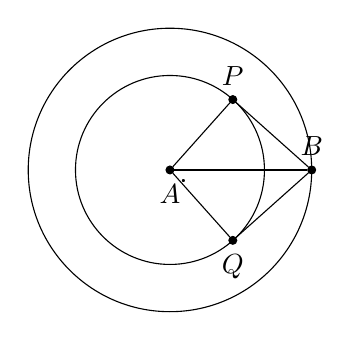
\begin{tikzpicture}
[scale =0.3,>=stealth,point/.style = {draw, circle, fill = black, inner sep = 1pt},]
\node (A) at (0,0)[point,label=below :$A$] {};
\node (P) at (2.66,2.98)[point,label=above :$P$] {};
\node (B) at (6,0)[point,label=above :$B$] {};
\node (Q) at (2.66,-2.98)[point,label=below :$Q$] {};
\draw (0,0) node [below right] {.} circle (6);
\draw (0,0) node [below right] {.} circle (4);
\draw (B)--(A);
\draw (B)--(Q);
\draw (B)--(P);
\draw (A)--(P);
\draw (A)--(Q);



\end{tikzpicture}
\end{document}